\subsection{Integrated yields as a function of \SOPT}\label{Sec:IntYield}

The integrated double ratio over the full \pt range is presented in Fig.~\ref{Fig:Extrapolation}, for p,~\LA, and \XI. The fully integrated yields are obtained by extrapolating the measured \pt spectra for each particle species. Therefore, the systematic uncertainties shown in Fig.~\ref{Fig:Extrapolation} also account for the added uncertainty due to the extrapolation procedure. This added uncertainty is particle species dependent given the different measured \pt ranges for each particle species, particularly affecting the \LA yields, which, as shown in Tab.~\ref{Tab:S0bias}, can only be measured down to 1.0 \gev after \SOPT selection. 

The results demonstrate that the strange-hadron yield increases as a function of \SOPT, with indications of an ordering with strangeness content. In previous ALICE publications it was observed that in pp collisions at \s$= 13$ TeV the charge particle density, \dndeta, is a driving quantity for the enhancement of strange hadrons~\cite{Naturepaper}. For the results presented in Fig.~\ref{Fig:Extrapolation}, the \dndeta at midrapidity is restricted (see Fig.~\ref{Fig:CL1vsV0M}), which allows one to directly test if \SOPT is sensitive to strangeness enhancement. We find that the strangeness production is suppressed in events with jet-like topologies, and slightly enhanced in softer, isotropic event topologies. 


\begin{figure}[h!]
    \vspace{0.1cm}
    \centering
    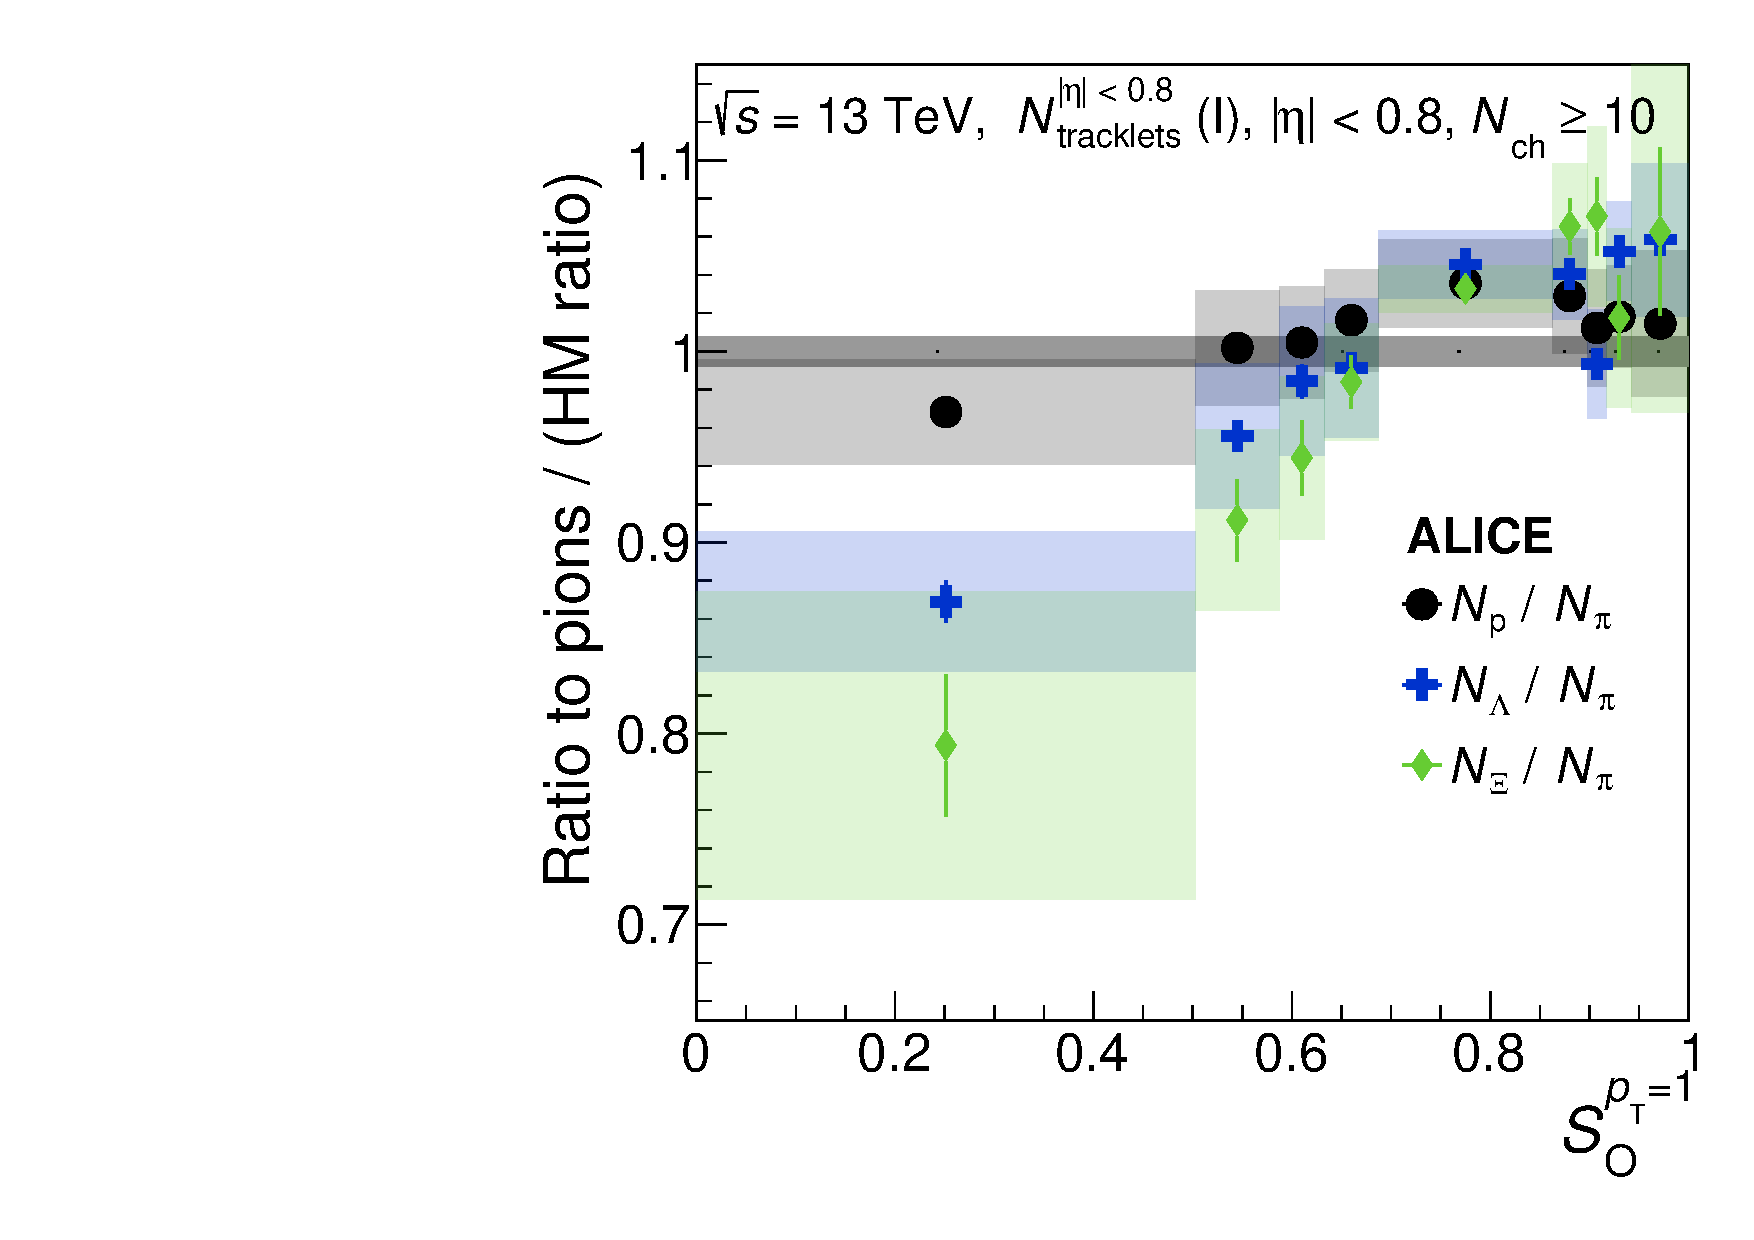
\includegraphics[scale=0.75]{figures/xi_over_pi_vs_So_CL1_01_EX.pdf}
    \caption{The double ratios of integrated yields as a function of \SOPT for the spectra of top-1\% \tracklet. The yield is estimated by extrapolating the spectra over the full \pt range. Statistical and systematic uncertainties are shown by bars and boxes, respectively. The grey band around unity represents the systematic uncertainty of the pion measurement.}
    \label{Fig:Extrapolation}
\end{figure}


In order to make the most precise comparison between the measured data and model predictions, the integrated double ratios are presented as a function of \SOPT for the measured \pt ranges in Fig.~\ref{Fig:CL1_1_Int_py} and Fig.~\ref{Fig:CL1_1_Int_hw}, for p,~\LA and \XI. The two figures contain the same data points, but use different ordinate ranges in the ratio to accommodate the MC-generator predictions. The yields for the measured \pt ranges are estimated by counting the bin entries in each \pt spectra, without the use of the Levy--Tsallis extrapolation. Therefore, the systematic uncertainties for the integrated yields utilizing the measured \pt ranges are significantly reduced compared to the extrapolated yields presented in Fig.~\ref{Fig:Extrapolation}. Moreover, while the fraction of yields gained from the extrapolation is species dependent, it was tested that the relative increase of yields is consistent across all spherocity classes and the high-multiplicity reference. As the integrated yields presented in Figs.~\ref{Fig:Extrapolation} --~\ref{Fig:CL1_1_Int_hw} are self-normalized, the relative yields obtained from the extrapolation therefore largely cancels. As such, one obtains the same physics conclusions by utilizing either extrapolated or measured \pt ranges, which is reflected in the comparison between Fig.~\ref{Fig:Extrapolation} and Fig.~\ref{Fig:CL1_1_Int_py}.

Figures ~\ref{Fig:CL1_1_Int_py} and ~\ref{Fig:CL1_1_Int_hw} highlight that the relative decrease of \XI production in the most jet-like events is of order 20\%. We estimate, based on Ref.~\cite{Naturepaper}, that to obtain a similar effect driven solely by multiplicity, one would have to decrease the multiplicity by approximately 60 to 70\%. Given that the difference in multiplicity between the spherocity event classes is roughly 10\%, this indicates a substantial lifting of the strangeness suppression due to the event topology selection.

\begin{figure}[th!]
    \vspace{0.1cm}
    \centering
    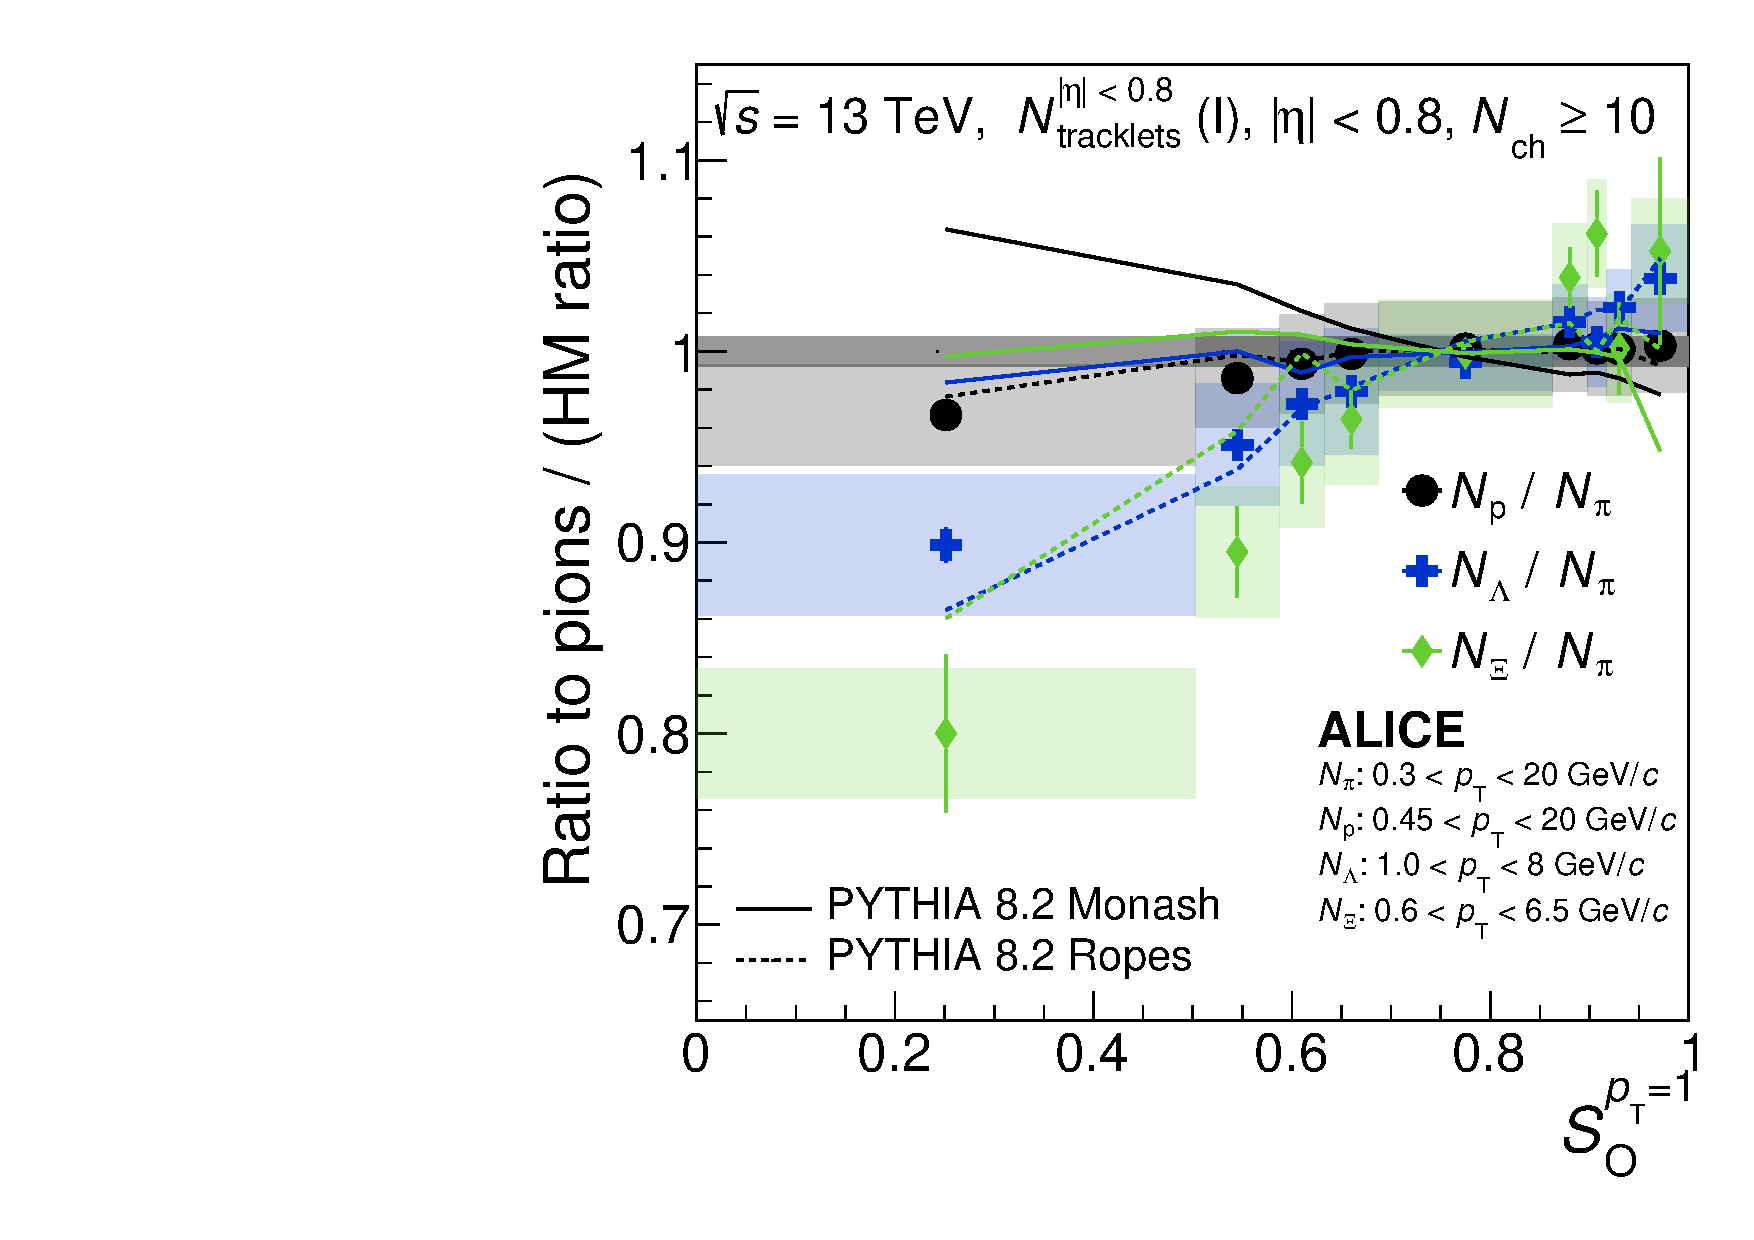
\includegraphics[scale=0.75]{figures/xi_over_pi_vs_So_CL1_01_PY.pdf}
    \caption{The double ratios of integrated yield as a function of \SOPT are represented in the top-1\% of \tracklet. The yields are integrated in the measured \pt ranges for each particle species. Statistical and systematic uncertainties are shown by bars and boxes, respectively. The curves represent different model predictions of the same measurement. The grey band around unity represents the systematic uncertainty of the pion measurement.}
    \label{Fig:CL1_1_Int_py}
\end{figure}

This novel feature can help to further elucidate the underlying mechanism(s) that drives the strangeness enhancement. Remarkably, these findings suggest that charged particle production is not driven by a single source, but instead driven by several sources with varying strangeness-to-\PI production rates, with the jet-like events showcasing a level of strangeness production usually found at lower multiplicities. In combination with the \pt-differential ratios from Figs.~\ref{Fig:CombRatioPy} --~\ref{Fig:CombRatioHerEx}, as well as the baryon-to-meson ratios in Fig.~\ref{Fig:Flow}, one can characterize jet-like events as exhibiting a large decrease of relative production at intermediate \pt, with an overall high degree of strangeness suppression in the total yields. Isotropic events can be characterized completely opposite to jet-like events, containing a boost of particles at intermediate \pt, with enhanced strangeness production in the \pt-integrated yields. These findings suggest that one is able to control the degree of QGP-like effects in small systems by categorizing events based on the azimuthal topology. Furthermore, it demonstrates that \SOPT-integrated high-multiplicity events are dominated by soft processes, and provides an important input to understanding the ALICE observation of universal scaling of strangeness enhancement with multiplicity~\cite{Naturepaper}.

\begin{figure}[t!]
    \vspace{0.1cm}
    \centering
    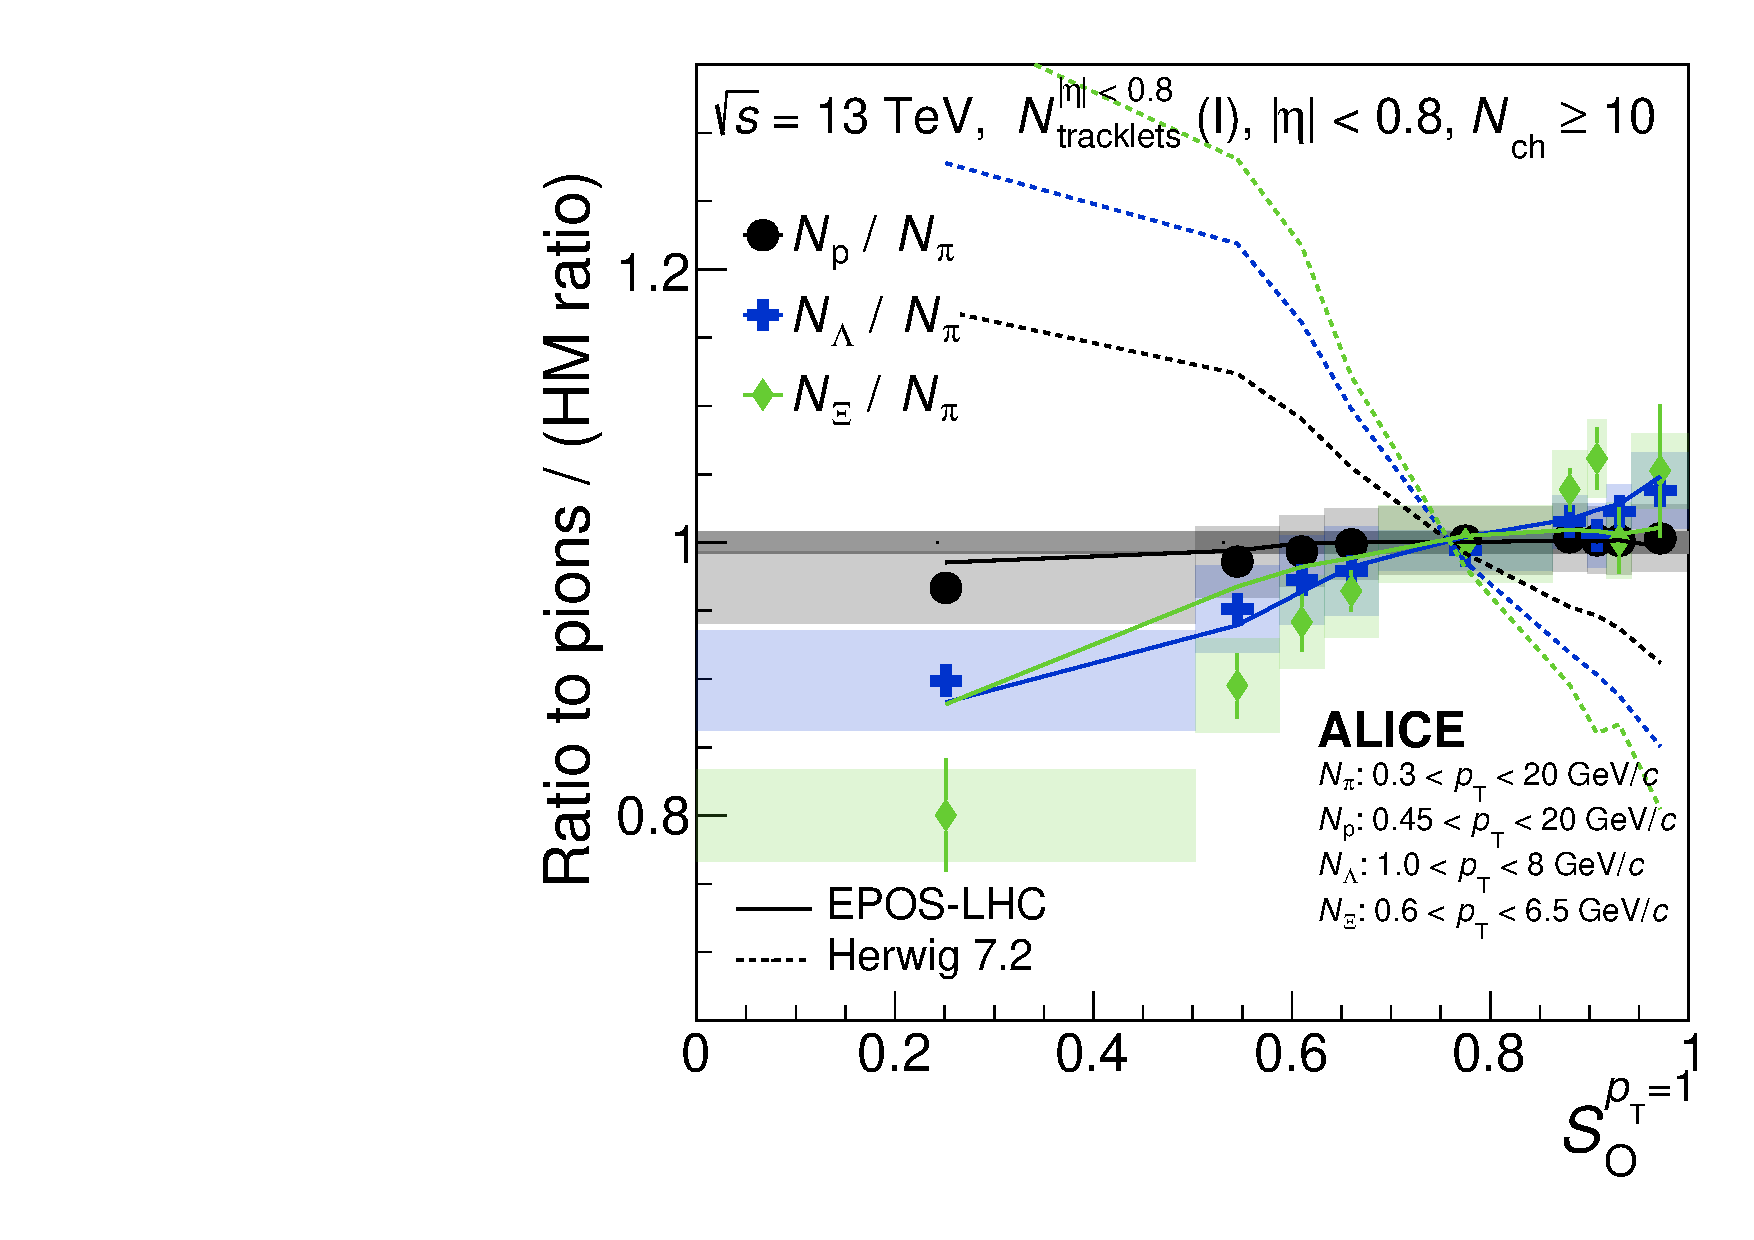
\includegraphics[scale=0.75]{figures/xi_over_pi_vs_So_CL1_01_HW.pdf}
    \caption{The double ratios of integrated yield as a function of \SOPT are represented in the top-1\% of \tracklet. The yields are integrated in measured \pt ranges for each particle species. Statistical and systematic uncertainties are shown by bars and boxes, respectively. Figure~\ref{Fig:CL1_1_Int_py} and Fig.~\ref{Fig:CL1_1_Int_hw} both contain the same experimental data, but the vertical ranges are modified to accommodate the model predictions. The curves represent different model predictions of the same measurement. The grey band around unity represents the systematic uncertainty of the pion measurement.}
    \label{Fig:CL1_1_Int_hw}
\end{figure}

The PYTHIA 8.2 Rope hadronization framework and EPOS-LHC models, which incorporate two-component phenomenologies, are able to predict the qualitative trend of enhancement and suppression of strange particle production as a function of \SOPT, albeit with a different mass-ordering for \LA and \XI. In contrast, both the PYTHIA8 Monash and Herwig 7.2 predictions are unable to describe the reported experimental observation. Surprisingly, Herwig 7.2 predicts the opposite trend; enhancement of all three baryons in jet-like events and a suppression in isotropic events. If this is a generic feature of the new strangeness-enhancement process introduced in Herwig 7.2\cite{Herwig}, then the results presented in this article appear to rule out this mechanism. Furthermore, it might seem counterintuitive that there can be large differences between model predictions in Fig.~\ref{Fig:CL1_1_Int_py} and Fig.~\ref{Fig:CL1_1_Int_hw}, while those same models had similar trends for the \pt-differential double-ratios presented in Figs.~\ref{Fig:CombRatioPy}--\ref{Fig:CombRatioHerEx}. However, it is important to note that the integrated double-ratios are weighted by the relative yields in each \pt interval. Therefore, the \mpt of each particle species play a major part in the integrated particle yields, see Fig.~\ref{Fig:Levy}.

The comparison between model and data suggests that models without a universal hadronization scheme, either through the core--corona in EPOS-LHC, or through the color ropes in PYTHIA 8.2, are able to qualitatively reproduce the observed trends. In contrast, the default PYTHIA 8.2 Monash variation, based on the concept of jet universality, is unable to capture the feature presented in the data. 
